\pdfminorversion=4
\documentclass[aspectratio=169]{beamer}

\mode<presentation>
{
  \usetheme{default}
  \usecolortheme{default}
  \usefonttheme{default}
  \setbeamertemplate{navigation symbols}{}
  \setbeamertemplate{caption}[numbered]
  \setbeamertemplate{footline}[frame number]  % or "page number"
  \setbeamercolor{frametitle}{fg=white}
  \setbeamercolor{footline}{fg=black}
} 

\usepackage[english]{babel}
\usepackage[utf8x]{inputenc}
\usepackage{tikz}
\usepackage{courier}
\usepackage{array}
\usepackage{bold-extra}
\usepackage{minted}
\usepackage[thicklines]{cancel}
\usepackage{fancyvrb}

\xdefinecolor{dianablue}{rgb}{0.18,0.24,0.31}
\xdefinecolor{darkblue}{rgb}{0.1,0.1,0.7}
\xdefinecolor{darkgreen}{rgb}{0,0.5,0}
\xdefinecolor{darkgrey}{rgb}{0.35,0.35,0.35}
\xdefinecolor{darkorange}{rgb}{0.8,0.5,0}
\xdefinecolor{darkred}{rgb}{0.7,0,0}
\definecolor{darkgreen}{rgb}{0,0.6,0}
\definecolor{mauve}{rgb}{0.58,0,0.82}

\title[2019-05-09-physicsforum-languages]{Analysis Description Languages}
\author{Jim Pivarski}
\institute{Princeton University -- IRIS-HEP}
\date{May 9, 2019}

\usetikzlibrary{shapes.callouts}

\begin{document}

\logo{\pgfputat{\pgfxy(0.11, 7.4)}{\pgfbox[right,base]{\tikz{\filldraw[fill=dianablue, draw=none] (0 cm, 0 cm) rectangle (50 cm, 1 cm);}\mbox{\hspace{-8 cm}
\includegraphics[height=1 cm]{princeton-logo-long.png}\hspace{0.1 cm}\raisebox{0.1 cm}{
\includegraphics[height=0.8 cm]{iris-hep-logo-long.png}}\hspace{0.1 cm}}}}}

\begin{frame}
  \titlepage
\end{frame}

\logo{\pgfputat{\pgfxy(0.11, 7.4)}{\pgfbox[right,base]{\tikz{\filldraw[fill=dianablue, draw=none] (0 cm, 0 cm) rectangle (50 cm, 1 cm);}\mbox{\hspace{-8 cm}
\includegraphics[height=1 cm]{princeton-logo.png}\hspace{0.1 cm}\raisebox{0.1 cm}{
\includegraphics[height=0.8 cm]{iris-hep-logo.png}}\hspace{0.1 cm}}}}}

% Uncomment these lines for an automatically generated outline.
%\begin{frame}{Outline}
%  \tableofcontents
%\end{frame}

% START START START START START START START START START START START START START

%% \begin{frame}{}
%% \vspace{-0.25 cm}
%% \begin{columns}[t]
%% \column{1.15\linewidth}
%% 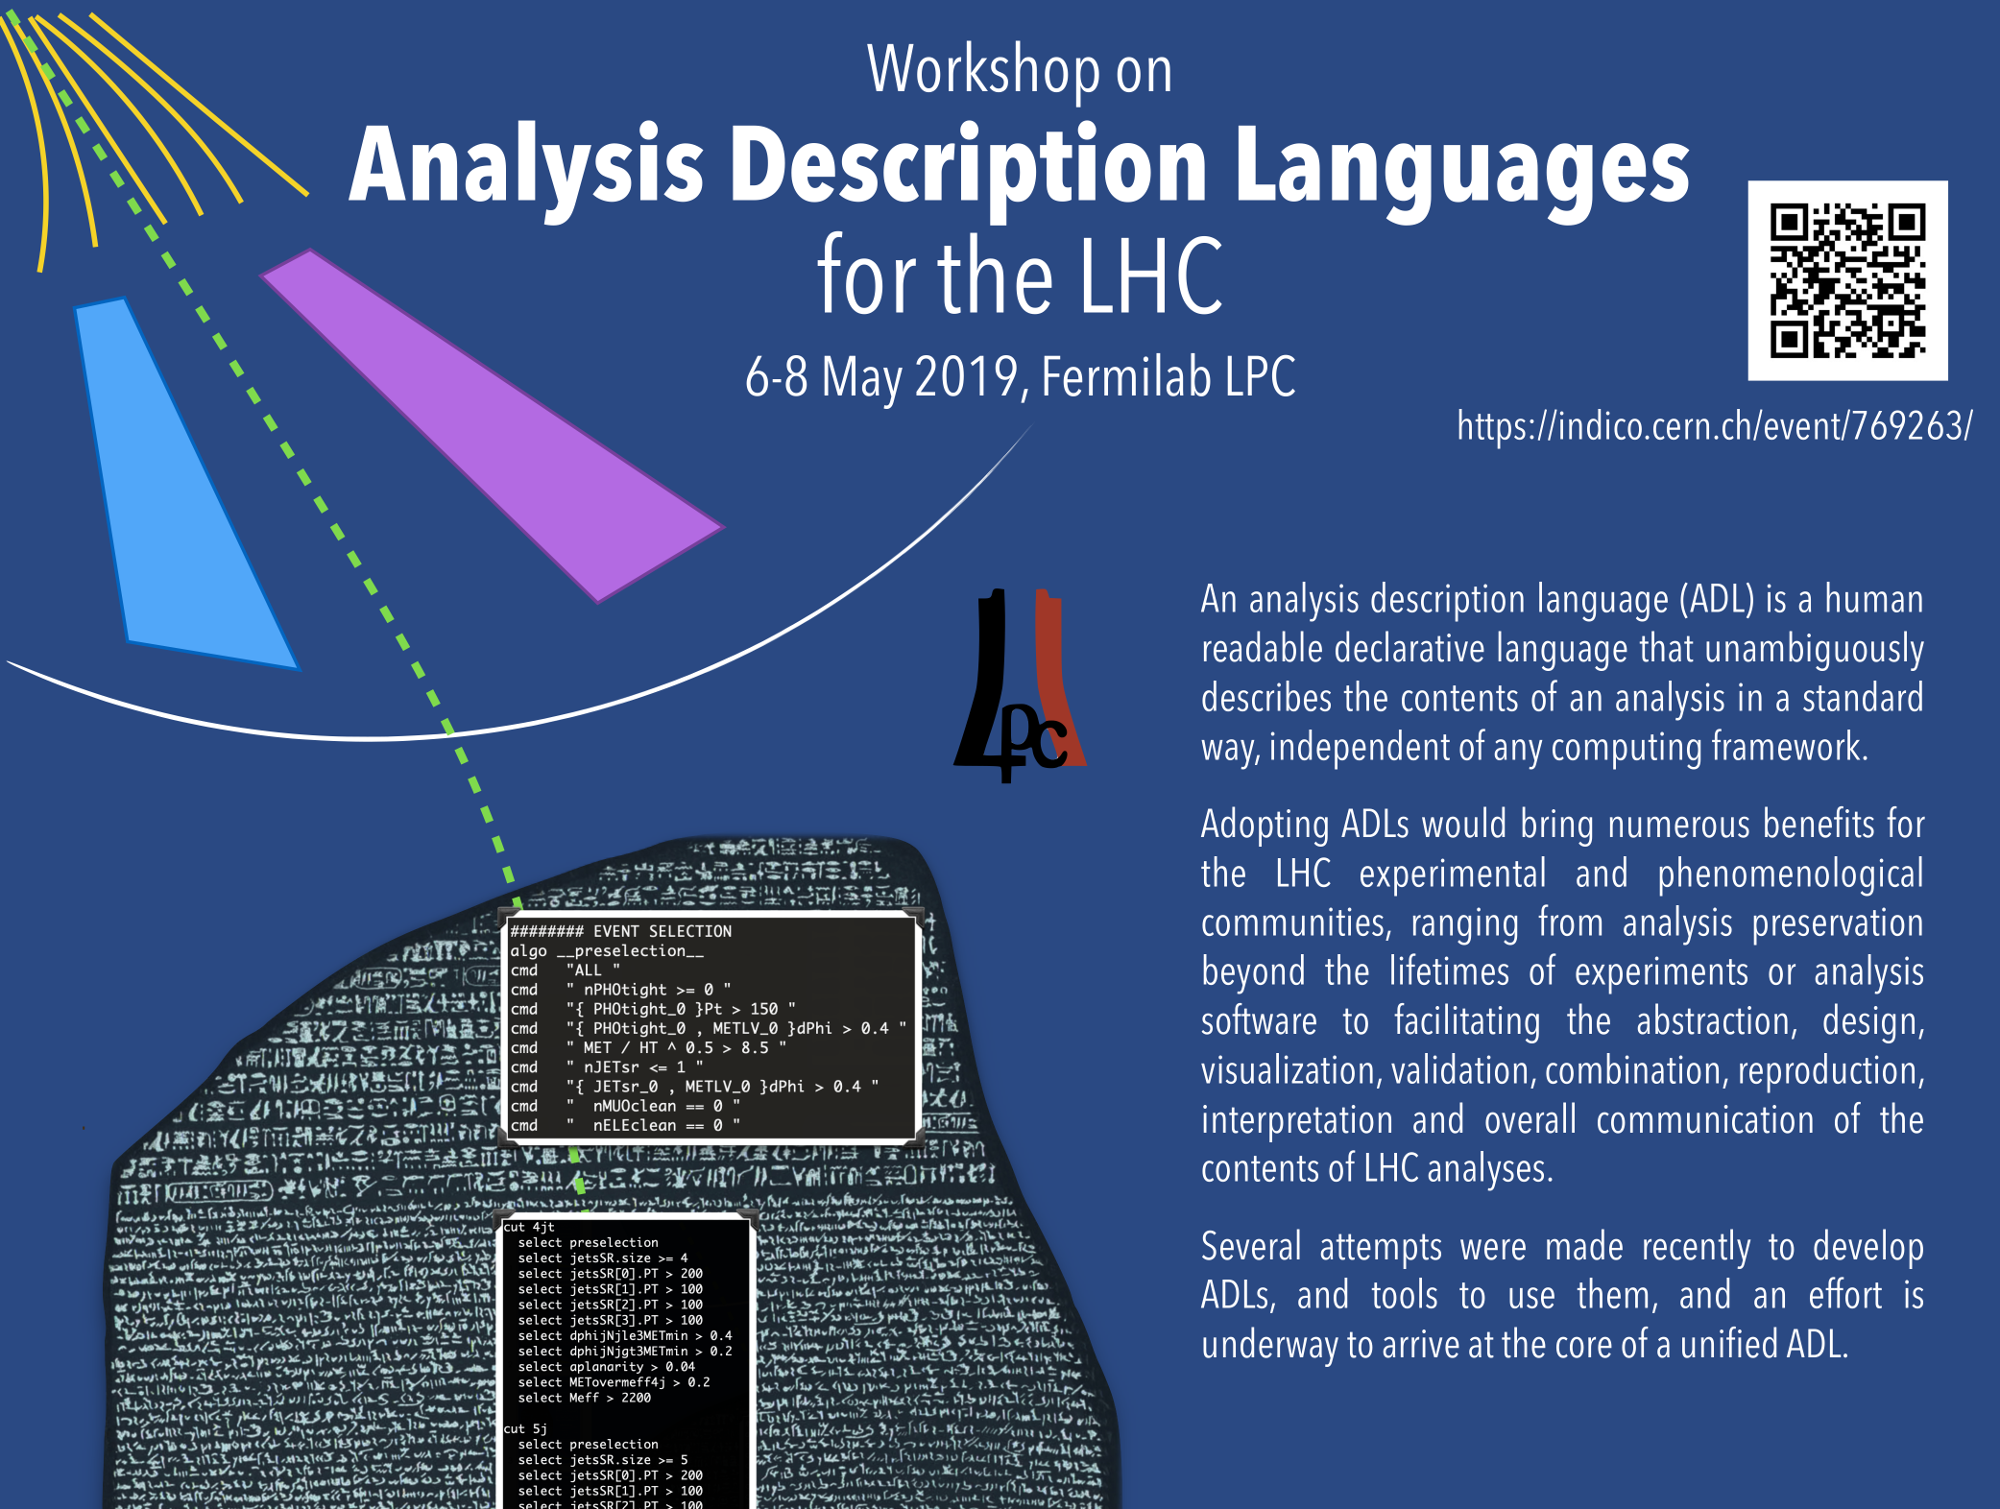
\includegraphics[width=\linewidth]{ADLposter_v3.png}
%% \end{columns}
%% \end{frame}

%% \begin{frame}{}
%% \LARGE
%% \vspace{1 cm}
%% \begin{block}{\huge Analysis Description Language}
%% A focused, limited language for some part of HEP analysis with physics concepts baked in.
%% \end{block}
%% \end{frame}

%% \begin{frame}{}
%% \begin{columns}[t]
%% \column{1.16\linewidth}
%% 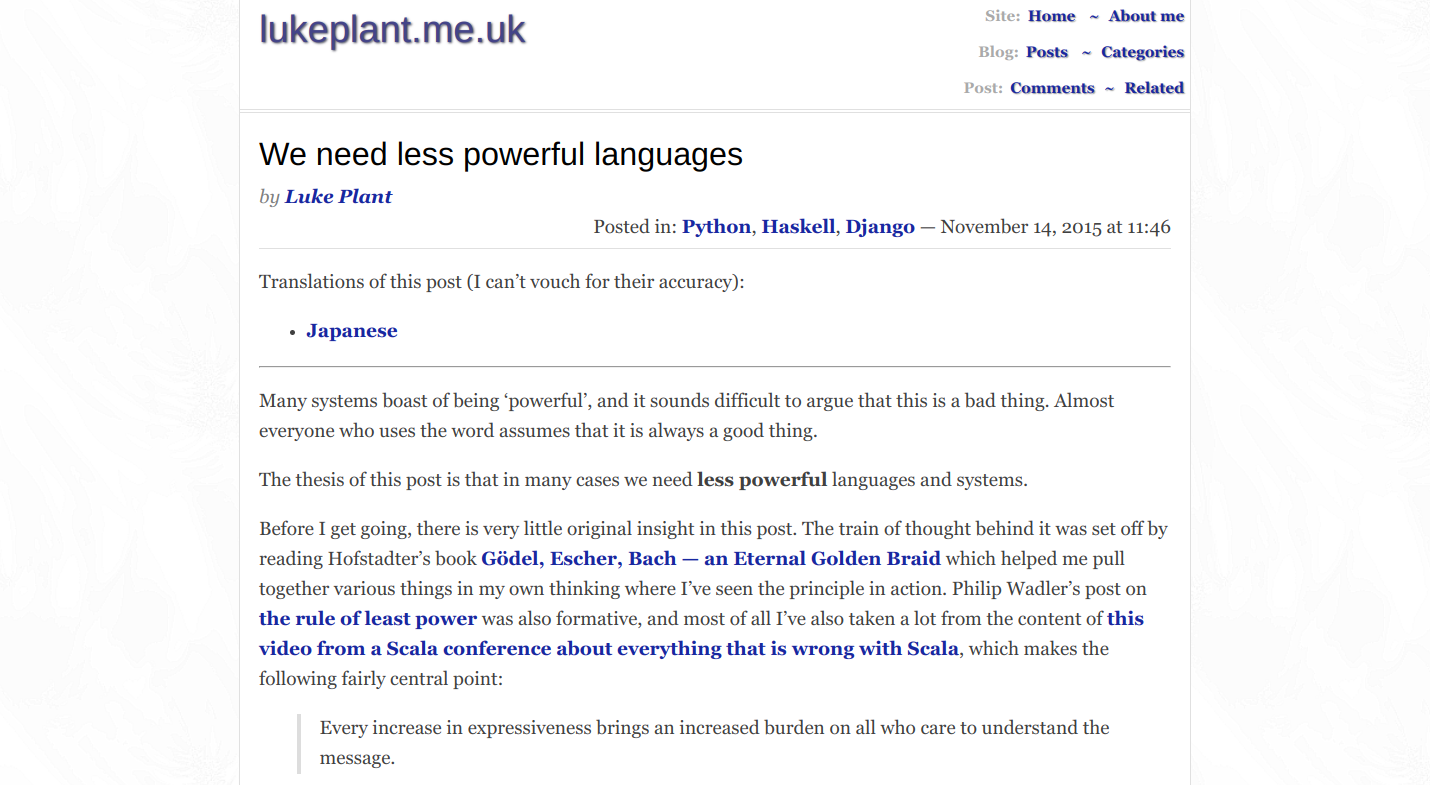
\includegraphics[width=\linewidth]{less-powerful.png}
%% \end{columns}
%% \end{frame}

%% \begin{frame}{}
%% \vspace{0.5 cm}
%% \LARGE
%% \begin{center}
%% Why would anyone want to use a limited language?
%% \end{center}
%% \end{frame}

%% \begin{frame}{The value of abstraction is known to physicists}
%% \large
%% \vspace{0.5 cm}
%% \begin{columns}
%% \column{0.25\linewidth}
%% 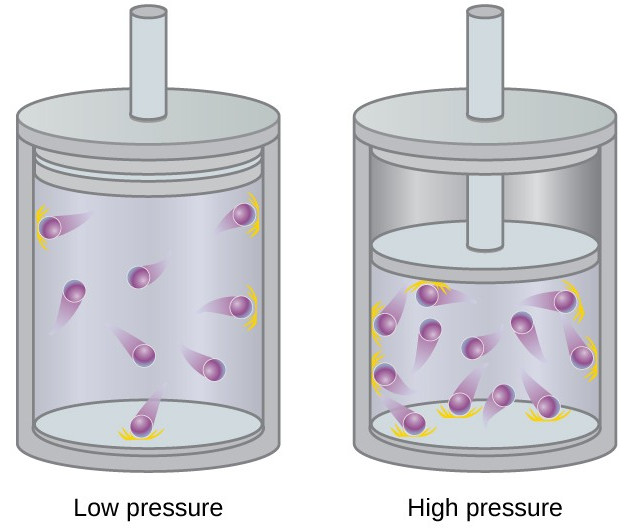
\includegraphics[width=\linewidth]{idealgas.jpg}

%% \column{0.6\linewidth}
%% \begin{block}{\LARGE Thermodynamics:}
%% \vspace{0.1 cm}
%% Replaces a problem of $\mathcal{O}(10^{24})$ free parameters

%% \vspace{0.1 cm}
%% with a problem of $\mathcal{O}(3)$ free parameters.
%% \end{block}
%% \end{columns}

%% \vspace{0.8 cm}
%% \begin{uncoverenv}<2->
%% \begin{columns}
%% \column{0.6\linewidth}
%% 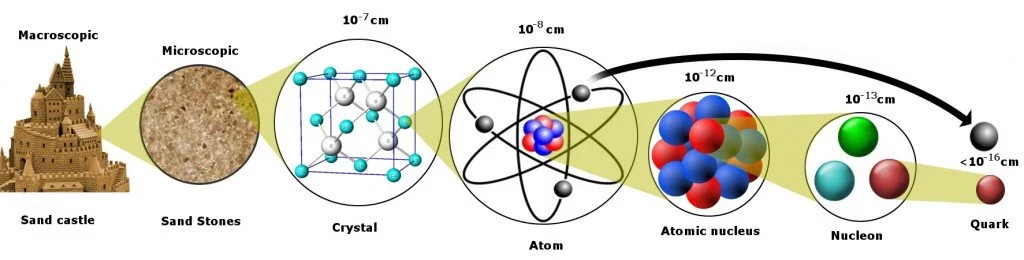
\includegraphics[width=\linewidth]{atom-proton-quark.png}

%% \column{0.3\linewidth}
%% \begin{block}{\LARGE Effective theories:}
%% \vspace{0.2 cm}
%% Allow you to focus on

%% \vspace{0.1 cm}
%% one problem at a time.
%% \end{block}
%% \end{columns}
%% \end{uncoverenv}
%% \end{frame}

%% \begin{frame}[fragile]{Much of computer science is about abstracting away details, too}
%% \scriptsize
%% \vspace{0.2 cm}
%% \begin{minted}{c++}
%% double bessel_j0(double x) {      // one value goes in...
%%     double out;
%%     if (fabs(x) < 8.0) {
%%         double y = x*x;
%%         double ans1 = 57568490574.0 + y*(-13362590354.0 + y*(651619640.7
%%                       + y*(-11214424.18 + y*(77392.33017 + y*(-184.9052456)))));
%%         double ans2 = 57568490411.0 + y*(1029532985.0 + y*(9494680.718
%%                       + y*(59272.64853 + y*(267.8532712 + y*1.0))));
%%         out = ans1 / ans2;
%%     }
%%     else {
%%         double z = 8.0 / fabs(x);
%%         double y = z*z;
%%         double xx = fabs(x) - 0.785398164;
%%         double ans1 = 1.0 + y*(-0.1098628627e-2 + y*(0.2734510407e-4
%%                       + y*(-0.2073370639e-5 + y*0.2093887211e-6)));
%%         double ans2 = -0.1562499995e-1 + y*(0.1430488765e-3
%%                       + y*(-0.6911147651e-5 + y*(0.7621095161e-6
%%                       - y*0.934935152e-7)));
%%         out = sqrt(0.636619772/fabs(x))*(cos(xx)*ans1 - z*sin(xx)*ans2);
%%     }
%%     return out;                   // ...one value comes out
%% }
%% \end{minted}
%% \end{frame}

%% \begin{frame}{Smaller numbers of external parameters are easier to think about}
%% \vspace{0.2 cm}
%% 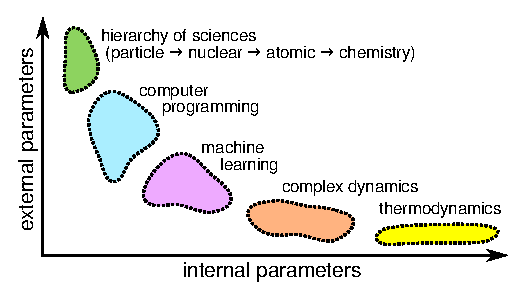
\includegraphics[width=\linewidth]{internal-vs-external.pdf}
%% \end{frame}

%% \begin{frame}{}
%% \large
%% \vspace{1 cm}
%% \begin{center}
%% A programming language has everything to do with making a calculation \\ easier to think about and nothing to do with making it happen.
%% \end{center}

%% \vspace{0.5 cm}
%% \begin{uncoverenv}<2->
%% \begin{columns}
%% \column{0.1\linewidth}

%% \column{0.35\linewidth}
%% \begin{center}
%% Making something happen by saying it is called magic.
%% \end{center}

%% \column{0.3\linewidth}
%% 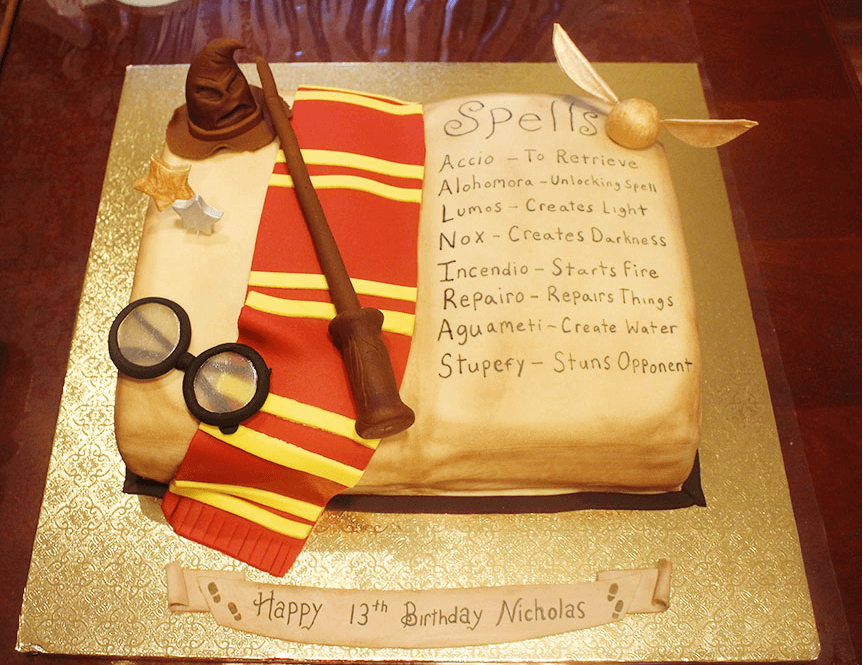
\includegraphics[width=\linewidth]{Harry-Potter-Cake.png}

%% \column{0.1\linewidth}
%% \end{columns}
%% \end{uncoverenv}
%% \end{frame}

%% \begin{frame}{Programming languages are human languages}
%% \vspace{0.25 cm}
%% \begin{itemize}
%% \item The computer is a set of physical states that we interpret as calculations.
%% \item We might have different languages to describe those calculations.
%% \item Some languages are better than others.
%% \end{itemize}

%% \begin{center}
%% 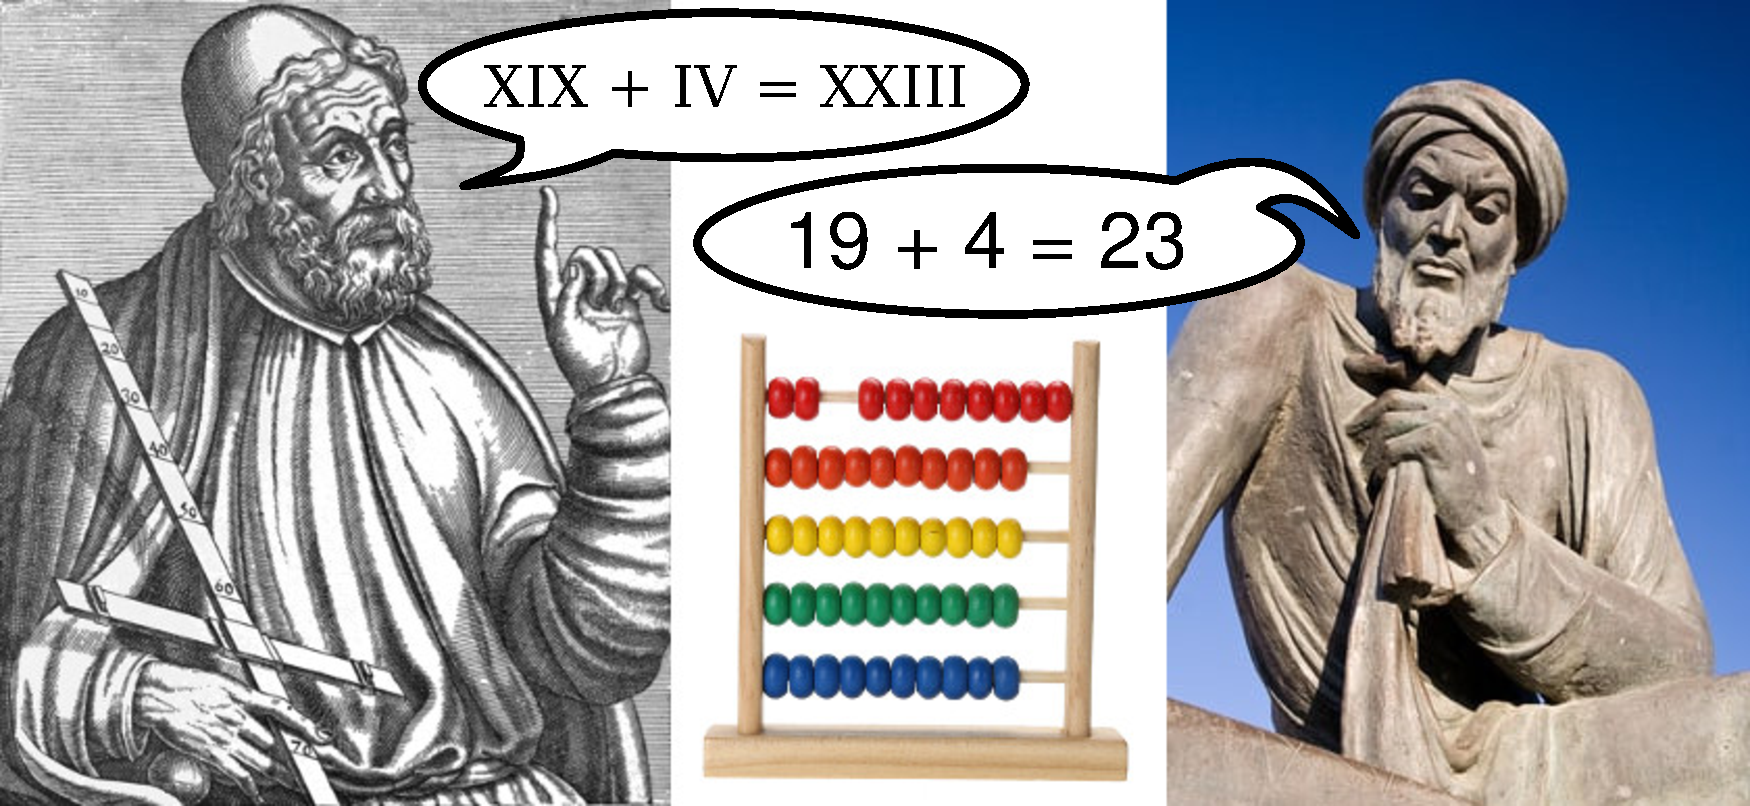
\includegraphics[width=0.9\linewidth]{abacus_ptolemy_al-khwarizmi.pdf}
%% \end{center}
%% \end{frame}

%% \begin{frame}{Originally, programming languages didn't move the abacus beans}
%% \vspace{0.25 cm}
%% \begin{columns}
%% \column{0.5\linewidth}
%% Ada Lovelace's algorithm for computing Bernoulli numbers was written for a computer that never ended up being invented.

%% \column{0.5\linewidth}
%% \hfill\mbox{\hspace{-1 cm}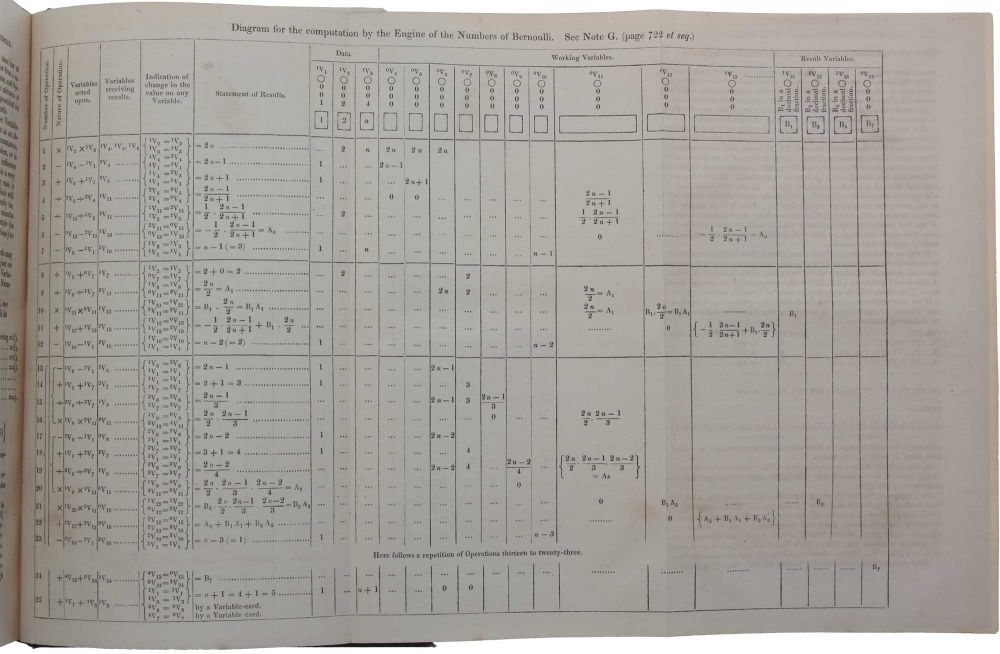
\includegraphics[height=3 cm]{ada-program.jpg}\hspace{0.5 cm}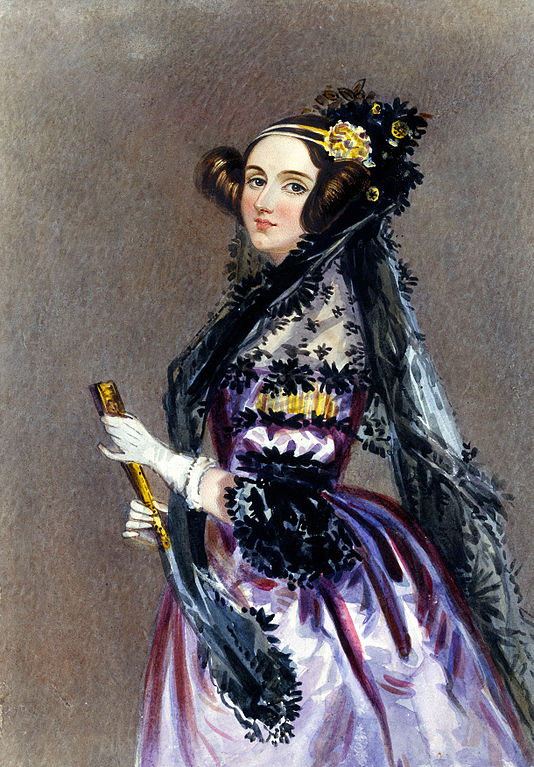
\includegraphics[height=3 cm]{ada.jpg}}
%% \end{columns}

%% \vspace{0.5 cm}
%% \begin{columns}
%% \column{1.05\linewidth}
%% \textcolor{darkblue}{John McCarthy, creator of Lisp:} ``This EVAL was written and published in the paper and Steve Russel said, `Look, why don't I program this EVAL?' and I said to him, `Ho, ho, you're confusing theory with practice---this EVAL is intended for reading, not for computing!' But he went ahead and did it.''
%% \end{columns}

%% \vspace{0.5 cm}
%% \begin{columns}
%% \column{1.05\linewidth}
%% \textcolor{darkblue}{APL (ancestor of MATLAB, R, and Numpy)} was also a notation for understanding computers years before it was executable. The book was named {\it A Programming Language}.
%% \end{columns}
%% \end{frame}

%% \begin{frame}{Once exclusively Fortran, HEP today uses C++ and Python}
%% \large
%% \vspace{0.5 cm}
%% \begin{center}
%% Languages of non-fork repos for GitHub users who also fork {\tt cms-sw/cmssw}
%% \end{center}

%% \vspace{-0.25 cm}
%% \begin{columns}
%% \column{1.3\linewidth}
%% \mbox{\hspace{-1 cm}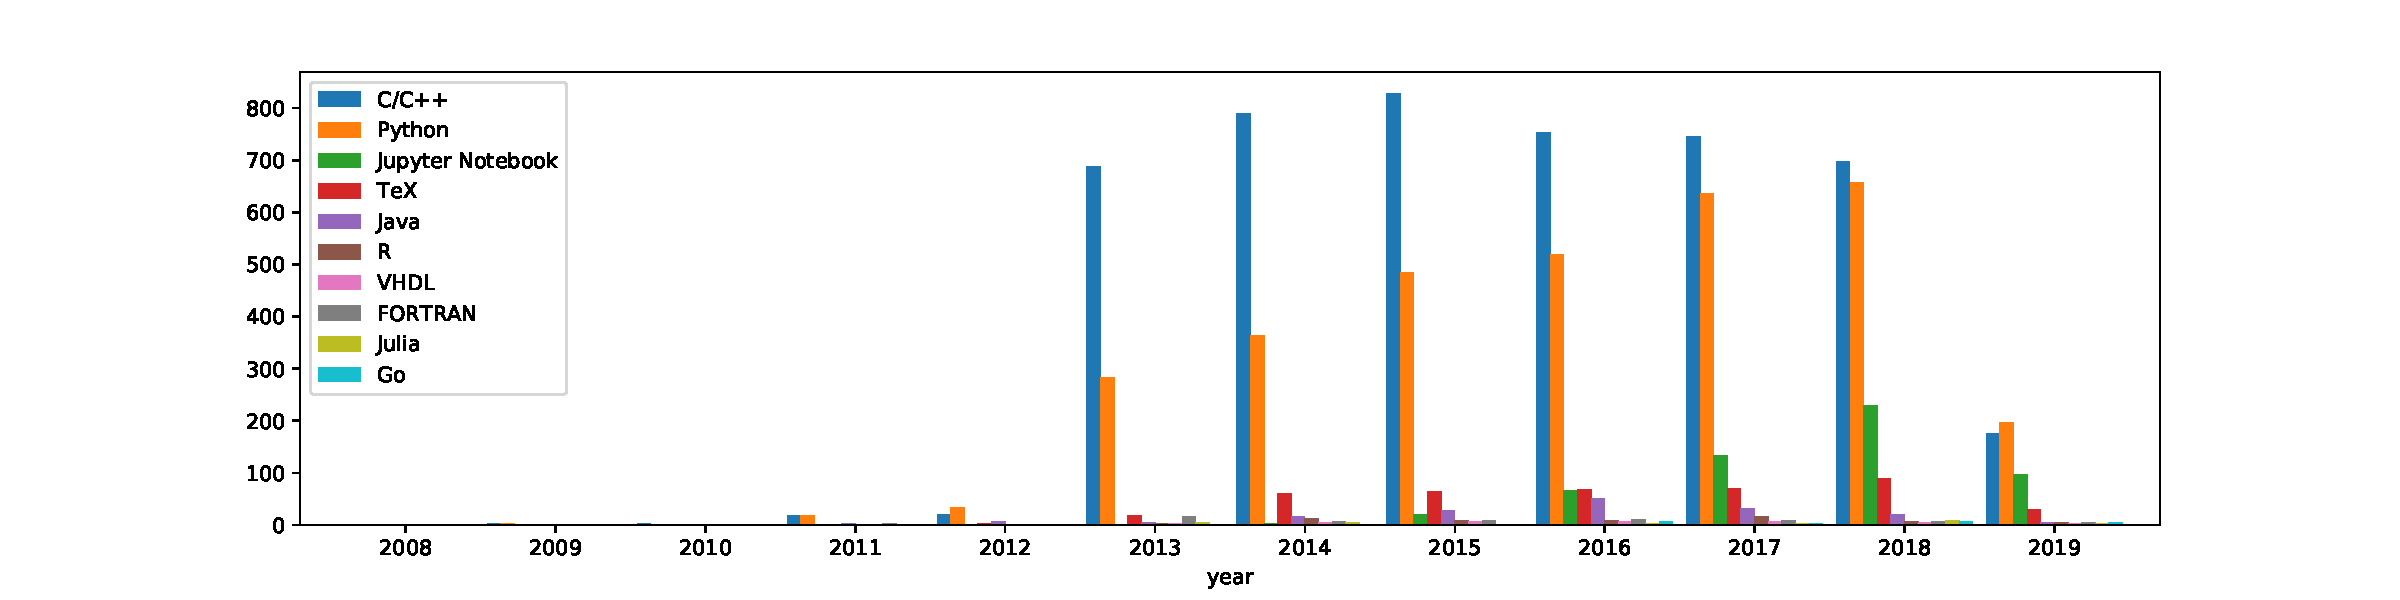
\includegraphics[width=\linewidth]{physicist-github-languages-lin.pdf}}
%% \end{columns}

%% \begin{center}
%% \textcolor{gray}{(The Fortran $\to$ C++ transition happened 20 years ago.)}
%% \end{center}
%% \end{frame}

%% \begin{frame}{Fortran, C++, and Python are general purpose machines}
%% \Large
%% \vspace{0.5 cm}
%% \begin{columns}
%% \column{1.1\linewidth}
%% \begin{center}
%% ``Did I fill that histogram before or after the \mintinline{python}{continue} statement?''
%% \end{center}
%% \end{columns}
%% \end{frame}

\begin{frame}[fragile]{}
\small
\begin{minted}{sql}
SELECT CONCAT(first, " ", last) AS fullname, AVG(age)
    FROM df WHERE age BETWEEN 18 AND 24
    GROUP BY fullname
\end{minted}

\begin{minted}{python}
>>> import pyspark.sql.functions as F

>>> (df.withColumn("fullname",
...         F.concat(F.col("first"), F.lit(" "), F.col("last")))
...    .select("fullname", "age")
...    .where(df.age.between(18, 24))
...    .groupBy("fullname")
...    .agg(F.mean("age")))
\end{minted}

\end{frame}



%% \begin{frame}{Maybe it goes back to origins? 1890 census: the Hollerith machine}
%% \vspace{0.25 cm}
%% \begin{center}
%% 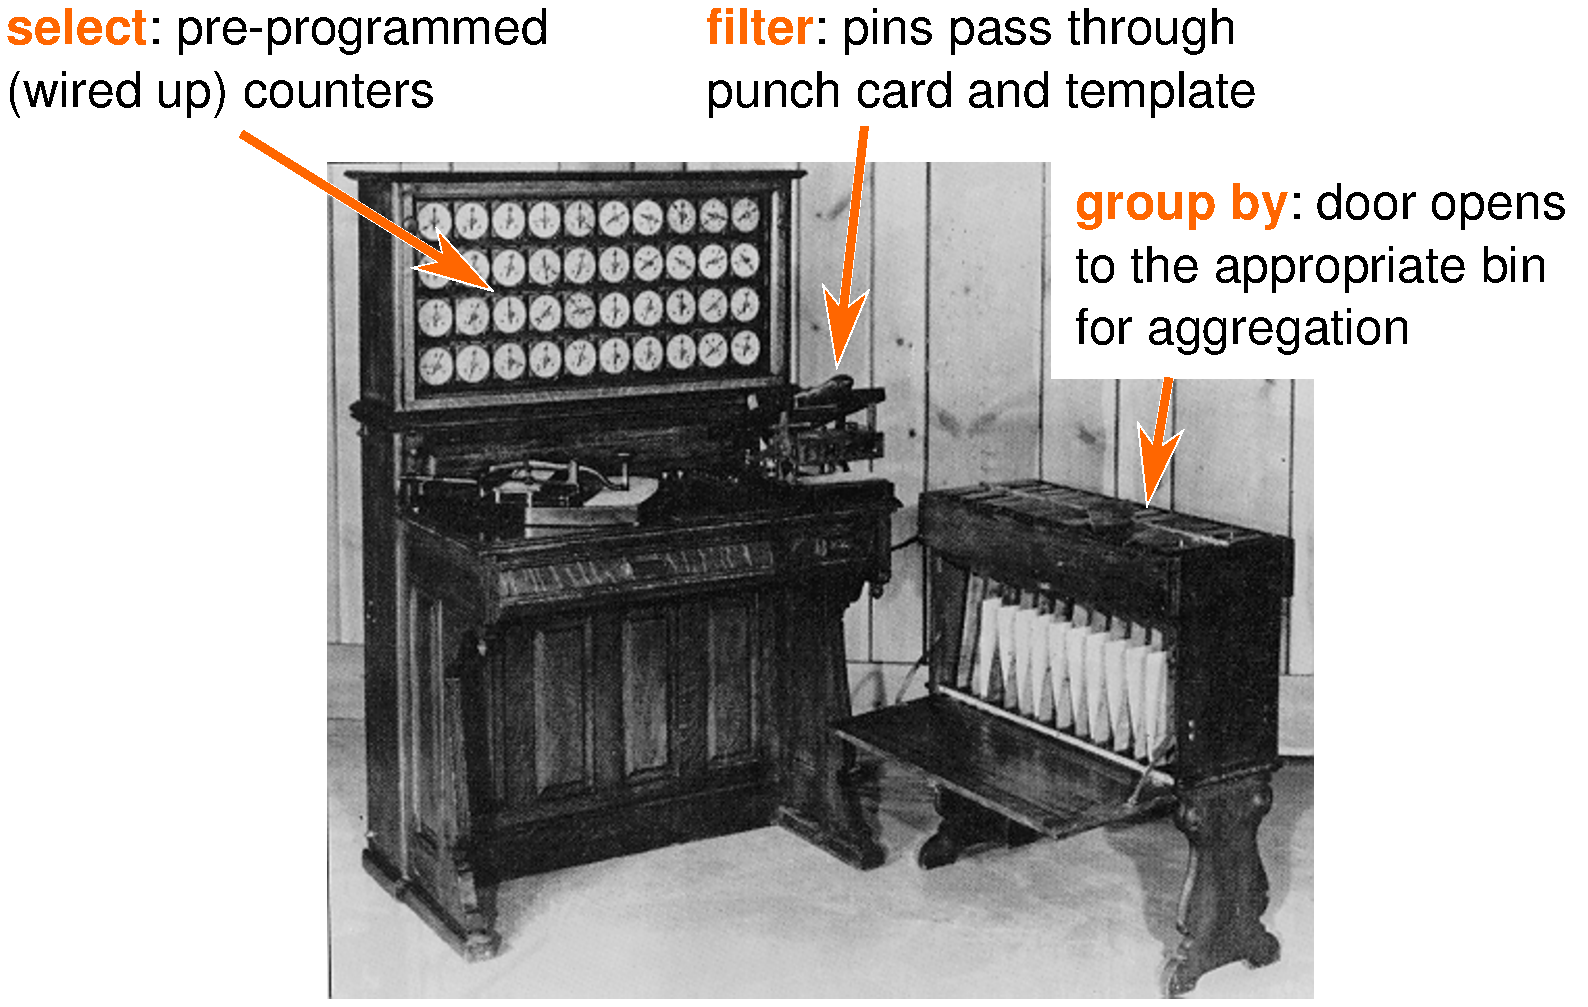
\includegraphics[width=0.83\linewidth]{hh-tabulator.pdf}
%% \end{center}
%% \end{frame}

%% \begin{frame}{Maybe it goes back to origins? 1950's neutron transport MC}
%% \vspace{0.5 cm}

%% 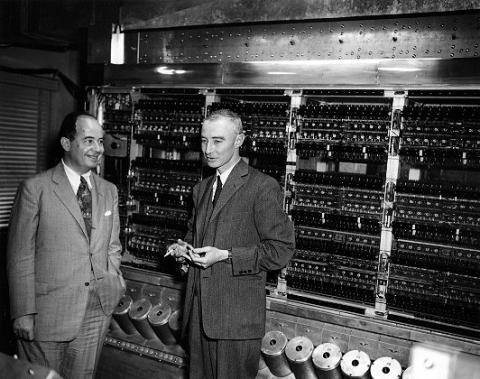
\includegraphics[height=5 cm]{neumann_oppie.jpg} 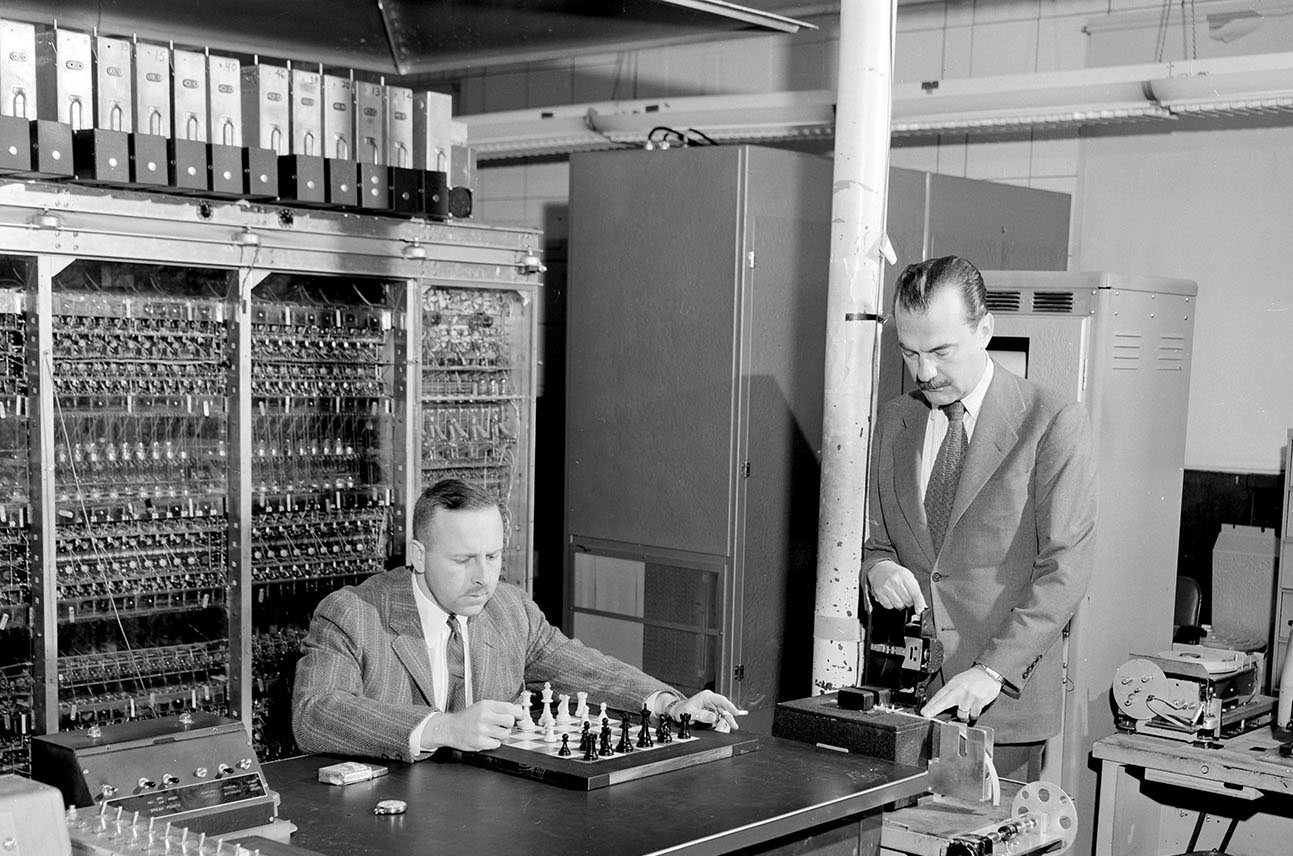
\includegraphics[height=5 cm]{metropolis.jpg}

%% \begin{center}
%% \Large {\bf M}etropolis {\bf A}nd {\bf N}eumann {\bf I}nvent {\bf A}wful {\bf C}ontraption
%% \end{center}
%% \end{frame}

\end{document}
